\documentclass[12pt]{article}
\usepackage[utf8]{inputenc} % Sin el guion
\usepackage[T1]{fontenc}    % Ayuda a que las tildes se copien bien del PDF
\usepackage[spanish]{babel}
\usepackage{amsmath}
\usepackage{amssymb}
\usepackage{geometry}
\usepackage[backend=biber,style=numeric]{biblatex}
\usepackage{csquotes}
\usepackage[table,xcdraw]{xcolor} 
\usepackage{tabularx}
\usepackage{subcaption}
\bibliography{referencias}
\geometry{margin=1in}
\usepackage{listings}
\usepackage{xcolor}

\usepackage{graphicx}
\usepackage{float}      % opcional, para usar [H]
\usepackage{hyperref}

\lstset{
    language=Python,
    basicstyle=\ttfamily\footnotesize,
    keywordstyle=\color{blue},
    commentstyle=\color{gray},
    stringstyle=\color{black},
    numbers=left,
    numberstyle=\tiny,
    frame=single,
    rulecolor=\color{black},
    breaklines=true,
    showstringspaces=false
}

\title{Actividad 5. Aprendizaje Automatico (KNN) e IDE3}
\author{Ing. Isaias Garcia Zanella}
\date{\today}

\begin{document}

\maketitle

\section{Introducción}

El aprendizaje automático es hoy uno de los pilares fundamentales de la inteligencia artificial moderna. A medida que la capacidad de cómputo crece y los conjuntos de datos disponibles se vuelven más extensos, los algoritmos capaces de aprender patrones a partir de la experiencia han ganado un papel protagónico en disciplinas tan diversas como la medicina, las finanzas, la ingeniería y las ciencias sociales.

En este contexto, el presente trabajo tiene como objetivo explorar e implementar desde cero dos de los algoritmos de aprendizaje automático más representativos: el algoritmo de \textbf{K-Vecinos más Cercanos (KNN)}, perteneciente al paradigma de aprendizaje basado en similitud, y el algoritmo \textbf{ID3}, perteneciente al paradigma de aprendizaje por árboles de decisión. Ambos enfoques representan estrategias conceptualmente distintas para abordar problemas de clasificación, y su estudio comparativo permite comprender de manera profunda los fundamentos del aprendizaje supervisado.

Para la implementación de KNN se utilizó el conjunto de datos \texttt{EnfCoronaria}, orientado a la predicción de enfermedades cardiacas, mientras que para ID3 se empleó el conjunto de datos \texttt{Titanic}. En ambos casos, los algoritmos fueron desarrollados sin el uso de bibliotecas especializadas de alto nivel, con el fin de fortalecer la comprensión de los principios matemáticos y computacionales que los sustentan.

El documento se organiza de la siguiente manera: primero se presenta el marco teórico que fundamenta ambos algoritmos; posteriormente se describen los materiales y métodos utilizados; luego se exponen y discuten los resultados obtenidos; y finalmente se presentan las conclusiones del trabajo.

\section{Marco Teórico}
\subsection{Aprendizaje Máquina}
La inteligencia artificial es un campo amplio de la informática que busca desarrollar sistemas capaces de realizar tareas que, si fueran llevadas a cabo por humanos, requerirían inteligencia. Estas tareas pueden incluir razonamiento, planificación, procesamiento del lenguaje natural, percepción visual, manipulación de objetos, toma de decisiones, entre muchas otras.
\\
Dentro de este gran campo, se encuentra el aprendizaje de máquinas (\textbf{machine learning}) como una de sus ramas más importantes. El aprendizaje de máquinas se enfoca en la capacidad del sistema de aprender y mejorar su rendimiento a partir de los datos, sin ser explícitamente programado para cada tarea.
\\
Una definición ampliamente aceptada y clara es la siguiente: <<El aprendizaje de máquinas es el campo que estudia cómo construir programas informáticos que puedan mejorar su rendimiento automáticamente mediante la experiencia>>. En ocasiones se maneja como sinónimo el término aprendizaje de máquinas con el aprendizaje automático. El aprendizaje automático tiene que ver con el etiquetado de los datos y es un tipo de aprendizaje de acuerdo a su supervisión.

\cite{De0a100enIA_2}

\subsection{Aprendizaje Basado en Similitud}

El aprendizaje basado en similitud en machine learning fundamenta su paradigma en el principio heurístico de que patrones históricos exitosos constituyen predictores confiables para instancias futuras. Es decir, el aprendizaje basado en similitud en lo que refiere a aprendizaje máquina tiene su origen en la idea de que la mejor manera de realizar una predicción o clasificación es simplemente observar lo que ha funcionado bien anteriormente y predecir el mismo comportamiento de nuevo. Las métricas más utilizadas son la euclidiana, Manhattan y Minkowski para este tipo de algoritmos.
\\
El modelo de aprendizaje máquina basado en similitud más popular es el algoritmo de K-Vecinos más Cercanos ---\textit{KNN} o \textit{K-Nearest Neighbors}---. Este también puede considerarse un modelo de clasificación.
\\
El algoritmo KNN implementa un enfoque de aprendizaje perezoso ---\textit{lazy learning}--- donde la fase de entrenamiento se reduce a almacenar el conjunto completo de instancias etiquetadas $D = \{(x_1,y_1), (x_2,y_2), \ldots, (x_n,y_n)\}$. Durante la inferencia, para una nueva instancia, el algoritmo ejecuta:
    \begin{enumerate}
        \item \textbf{Cálculo de distancia:} Computa $d(x_{\text{query}}, x_i)$ para todos los puntos de entrenamiento.
        \item \textbf{Selección de los $K$ vecinos más cercanos.}
        \item \textbf{Clasificación o predicción} basada en la votación mayoritaria (para clasificación) o el promedio (para regresión).
    \end{enumerate}

La selección del valor de $k$ presenta un balance fundamental entre sesgo y varianza:
\\
\textbf{$K$ pequeño ($k \to 1$):} Alta varianza, bajo sesgo. El modelo se vuelve sensible al ruido y puede sobreajustarse, generando fronteras de decisión irregulares.
\\
\textbf{$K$ grande ($k \to n$):} Baja varianza, alto sesgo. El modelo tiende a suavizar las fronteras de decisión, pudiendo perder patrones locales importantes.
\\
Este paradigma de aprendizaje encuentra aplicaciones exitosas en sistemas de recomendación, reconocimiento de patrones, análisis de series temporales y detección de anomalías, donde la interpretabilidad y la simplicidad conceptual son valoradas junto con la efectividad predictiva.

\cite{De0a100enIA}

\subsection{Aprendizaje por Árboles de Decisión}
Los árboles de decisión son de los algoritmos de aprendizaje máquina más usados en la historia. Son estructuras jerárquicas que imitan el proceso de toma de decisiones humano, dividiendo los datos de manera recursiva basándose en características específicas hasta llegar a una decisión final. Este algoritmo representa el conocimiento en forma de un árbol invertido, donde cada nodo interno representa una prueba sobre un atributo, cada rama representa una decisión y cada hoja representa una etiqueta de clase o un valor numérico.
\\
La construcción de un árbol de decisión es relativamente simple: cada nodo representa una característica, cada rama representa una decisión y cada hoja representa una salida (categórica o un valor continuo).
\\
Los árboles de decisión son versátiles y se utilizan tanto para problemas de clasificación como para regresión. Una de las preguntas primordiales es la razón por la cual usar árboles de decisión. La respuesta es simple: tienen varias ventajas respecto a otros métodos de aprendizaje máquina, como lo son:
\begin{itemize}
    \item \textbf{Interpretabilidad y transparencia:} Los árboles de decisión son fáciles de entender y visualizar, lo que los hace ideales para la interpretación de modelos.
    \item \textbf{Capacidad predictiva:} Los árboles de decisión se entrenan con instancias de ejemplos ya vistos y son capaces de predecir circunstancias no previstas anteriormente. Tampoco requieren suposiciones sobre la distribución de los datos.
    \item \textbf{Eficiencia computacional:} La construcción de un árbol de decisión es relativamente rápida, especialmente con algoritmos optimizados como ID3.
\end{itemize}

A pesar de sus ventajas, los árboles de decisión también presentan algunas limitaciones importantes:
\begin{itemize}
    \item \textbf{Sobreajuste:} Los árboles de decisión pueden ser propensos a sobreajustar los datos de entrenamiento, especialmente si el árbol es muy profundo.
    \item \textbf{Sesgo hacia atributos con muchas categorías:} Los árboles de decisión pueden favorecer atributos con un gran número de categorías, lo que puede llevar a modelos menos generalizables.
    \item \textbf{Problemas con clases desbalanceadas:} Los árboles de decisión pueden tener dificultades para manejar conjuntos de datos con clases desbalanceadas, lo que puede resultar en un rendimiento deficiente para la clase minoritaria.
    \item \textbf{Limitaciones de rendimiento:} En algunos casos, los árboles de decisión pueden no ser tan precisos como otros algoritmos de aprendizaje máquina, especialmente en problemas complejos con muchas interacciones entre características.
\end{itemize}

Existen varios algoritmos para construir un árbol de decisión. Dos de los más utilizados son:
\begin{itemize}
    \item \textbf{CART (Classification and Regression Trees):}
    \begin{itemize}
        \item \textit{Versatilidad:} Puede manejar tanto problemas de clasificación como de regresión.
        \item \textit{División binaria:} Siempre divide los nodos en dos ramas.
        \item \textit{Criterios de división:} Utiliza el índice Gini para clasificación y el error cuadrático medio para regresión.
        \item \textit{Poda:} Incluye técnicas de poda para evitar el sobreajuste.
    \end{itemize}
    \item \textbf{ID3 (Iterative Dichotomiser 3):}
    \begin{itemize}
        \item \textit{Enfoque en la clasificación:} Diseñado específicamente para problemas de clasificación.
        \item \textit{División múltiple:} Puede crear múltiples ramas por nodo.
        \item \textit{Criterio de información:} Usa ganancia de información basada en entropía.
        \item \textit{Simplicidad:} Algoritmo más simple pero efectivo.
    \end{itemize}
\end{itemize}

Otros algoritmos importantes de árboles de decisión son:
\begin{itemize}
    \item \textbf{C4.5:} Es una extensión de ID3 que maneja tanto atributos continuos como discretos, y utiliza el índice de ganancia de información normalizada.
    \item \textbf{CHAID (Chi-squared Automatic Interaction Detector):} Utiliza pruebas de chi-cuadrado para determinar las divisiones, y es especialmente efectivo para variables categóricas.
    \item \textbf{Random Forest:} Es un conjunto (\textit{ensemble}) de árboles de decisión que mejora la precisión y reduce el sobreajuste al promediar las predicciones de múltiples árboles construidos con subconjuntos aleatorios de los datos.
\end{itemize}

\cite{De0a100enIA_3}

\section{Materiales y Métodos}
\subsection{Herramientas y Entorno de Desarrollo}

Para el desarrollo de este proyecto se seleccionó un ecosistema de herramientas basado en el lenguaje Python, orientado específicamente al análisis de datos y el aprendizaje automático.

\subsubsection{Entorno de Ejecución}
\begin{itemize}
    \item \textbf{IDE:} Visual Studio Code (VS Code).
    \item \textbf{Formato:} Jupyter Notebook (\texttt{.ipynb}), el cual permite una ejecución interactiva y modular del código.
    \item \textbf{Lenguaje:} Python versión 3.14.2 (entorno local).
\end{itemize}

\subsubsection{Librerías y Dependencias}
A continuación se describen las librerías utilizadas y su función específica dentro del flujo de trabajo:

\begin{table}[H]
\renewcommand{\arraystretch}{1.5}
\centering
\begin{tabularx}{\textwidth}{|l|X|}
\hline
\rowcolor[HTML]{EFEFEF}
\textbf{Librería / Módulo} & \textbf{Descripción y Uso en el Proyecto} \\ \hline
\texttt{numpy} (np) & Soporte para vectores y matrices, esencial para los cálculos matemáticos de los modelos. \\ \hline
\texttt{pandas} (pd) & Manipulación y limpieza de estructuras de datos (DataFrames). \\ \hline
\texttt{seaborn} (sns) & Visualización estadística de datos y creación de gráficos de alta fidelidad. \\ \hline
\texttt{matplotlib} (plt) & Generación de gráficas base y control de la interfaz de trazado. \\ \hline
\end{tabularx}
\caption{Resumen de herramientas tecnológicas y librerías de Python utilizadas.}
\end{table}

En esta práctica se implementaron los algoritmos KNN e ID3 desde cero, sin utilizar librerías específicas de machine learning como \texttt{scikit-learn}, con el objetivo de comprender a fondo su funcionamiento interno y los principios matemáticos que los sustentan.
\\
Las bases de datos utilizadas para la implementación de ambos algoritmos fueron:
\begin{enumerate}
    \item \textbf{KNN:} Se utilizó el conjunto de datos \texttt{EnfCoronaria}, un dataset sintético que contiene información sobre pacientes con características clínicas relevantes para la predicción de enfermedades coronarias. Este dataset incluye atributos como edad, presión arterial, colesterol, entre otros, y una etiqueta binaria que indica la presencia o ausencia de enfermedad coronaria.
    \item \textbf{ID3:} Se empleó el conjunto de datos \texttt{Titanic}, un dataset basado en los sobrevivientes del Titanic, utilizado previamente en el examen realizado anteriormente.
\end{enumerate}

\section{Resultados y Discusión}
\subsection{KNN}
\subsubsection{Análisis de Resultados: Dataset Heart Disease}
El modelo \textit{myKNN} fue entrenado con una muestra de 370 pacientes, evaluando su desempeño sobre un conjunto de prueba de 92 individuos. Mediante un proceso de optimización iterativa, se determinó que un valor de $k=20$ vecinos proporciona el mejor balance entre sesgo y varianza, alcanzando una precisión del 70.27\%.

Visualmente, el clasificador logra delimitar las fronteras de decisión entre pacientes sanos y aquellos con patologías cardiacas. No obstante, el solapamiento observado en los diagramas de dispersión sugiere que la naturaleza multivariante del problema presenta casos donde los parámetros físicos son limítrofes, justificando el margen de error del 29.73\% observado en la validación cruzada.
\begin{figure}[H]
     \centering
     \begin{subfigure}[b]{0.8\textwidth}
         \centering
         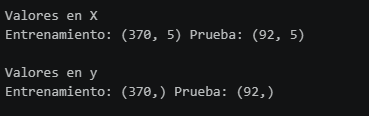
\includegraphics[width=\textwidth]{../Imagenes/Tarea5/DatosDivididosKNN.png}
         \caption{División de los datos en entrenamiento y prueba.}
     \end{subfigure}
     \hfill
     \begin{subfigure}[b]{0.8\textwidth}
         \centering
         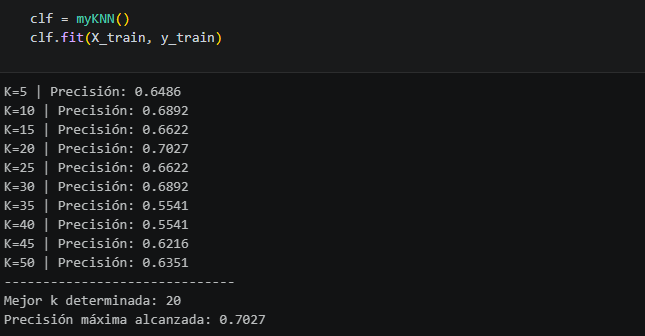
\includegraphics[width=\textwidth]{../Imagenes/Tarea5/K_Optimo.png}
         \caption{Búsqueda del $K$ óptimo.}
     \end{subfigure}
     \hfill
     \begin{subfigure}[b]{0.8\textwidth}
         \centering
         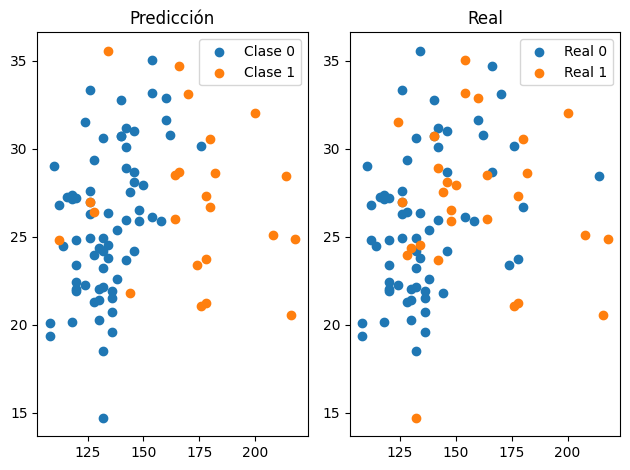
\includegraphics[width=\textwidth]{../Imagenes/Tarea5/Salida.png}
         \caption{Visualización de la clase real y la predicha.}
     \end{subfigure}
     \caption{Resultados obtenidos con el algoritmo KNN.}
     \label{fig:VisualizacionErrorOpen}
\end{figure}

\subsection{ID3}
\subsubsection{Comparativa de Modelos: Sklearn vs.\ ID3}
Mientras que el modelo de \textit{sklearn} genera un árbol binario balanceado y generalista, el algoritmo \textit{ID3} produce un árbol altamente ramificado basado en valores nominales y numéricos exactos.

La raíz del árbol ID3 es la variable \texttt{fare}, lo que sugiere que el nivel socioeconómico fue el factor con mayor ganancia de información inicial. Sin embargo, la presencia de nodos para valores de edad muy específicos (p.\,ej., 29.88) indica un fenómeno de sobreajuste que podría limitar la capacidad de generalización del modelo en comparación con la versión de \textit{sklearn}.

\section{Conclusión}

A lo largo de este trabajo se implementaron y evaluaron dos de los algoritmos de aprendizaje automático más representativos del aprendizaje supervisado: KNN e ID3. Su desarrollo desde cero permitió no solo comprender los principios matemáticos que los sustentan, sino también identificar con claridad sus fortalezas, limitaciones y el comportamiento práctico que exhiben ante conjuntos de datos reales.

En el caso del algoritmo KNN aplicado al dataset \texttt{EnfCoronaria}, se obtuvo una precisión del 70.27\% con un valor óptimo de $k=20$. Este resultado refleja el balance característico entre sesgo y varianza que impone la elección del hiperparámetro $k$: valores pequeños generan modelos sensibles al ruido, mientras que valores grandes tienden a suavizar en exceso las fronteras de decisión. El solapamiento observado en los datos sugiere que la separabilidad lineal del problema es limitada, lo cual es un factor inherente a la complejidad clínica de la predicción de enfermedades coronarias.

Por su parte, el algoritmo ID3 aplicado al dataset \texttt{Titanic} produjo un árbol altamente ramificado cuya raíz fue la variable \texttt{fare}, indicando que el nivel socioeconómico del pasajero fue el atributo con mayor poder discriminativo. Sin embargo, la aparición de nodos con valores de edad extremadamente específicos evidenció un sobreajuste al conjunto de entrenamiento, limitando la capacidad de generalización del modelo en comparación con la implementación de \textit{sklearn}, que genera árboles binarios más equilibrados mediante criterios de poda.

En términos comparativos, ambos algoritmos demostraron ser herramientas conceptualmente accesibles y computacionalmente eficientes, adecuadas para tareas de clasificación donde la interpretabilidad del modelo es prioritaria. No obstante, sus limitaciones ---especialmente el sobreajuste en ID3 y la sensibilidad al valor de $k$ en KNN--- subrayan la importancia de técnicas complementarias como la validación cruzada, la poda de árboles y el uso de métodos de ensamble como Random Forest.

Finalmente, la implementación manual de estos algoritmos constituyó un ejercicio valioso para consolidar la comprensión de los fundamentos del aprendizaje automático, sentando las bases para el estudio de modelos más complejos y robustos en etapas posteriores.

\printbibliography[title={Referencias Bibliográficas}]
\end{document}